\documentclass[a4paper,12pt]{report}

\usepackage[russian]{config}

\usepackage{minted}


% Description

\newcommand{\authorNameRu}{Маев Сергей Иванович}
\newcommand{\thesisTitleRu}{Изучение LaTeX и Git}
\newcommand{\thesisTypeRu}{Практическая}
\newcommand{\programulDeStudiiRu}{бакалавриата} 
\newcommand{\identificatorulCursuluiRu}{Информатика}
\newcommand{\conducatorNameRu}{Фамилия Имя}
\newcommand{\uniGroupName}{I2402}

\renewcommand{\year}{2025}
\newcommand{\github}{\url{https://github.com/USER/REPO}}
\newcommand{\outputDate}{\today}

\begin{document}

\begin{titlepage}
  \vspace*{\fill}
  \begin{center}
    \vspace*{1cm}

    \large
    \uppercase{\textbf{МОЛДАВСКИЙ ГОСУДАРСТВЕННЫЙ УНИВЕРСИТЕТ  \\}}

    \normalsize
    \uppercase{\textbf{ФАКУЛЬТЕТ МАТЕМАТИКИ И ИНФОРМАТИКИ}}
    \vspace{0.1cm}

    \normalsize
    \uppercase{\textbf{ДЕПАРТАМЕНТ ИНФОРМАТИКИ}}
    \vspace{3.0cm}

    \large
    \textbf{\correctName{\authorNameRu}}
    \vspace{1.5cm}

    \Large
    \textbf{\MakeUppercase{\thesisTitleRu}}
    \vspace{0.75cm}

    \large
    \textbf{\MakeUppercase{\identificatorulCursuluiRu}}
    \vspace{0.5cm}

    \normalsize
    \textbf{\expandafter\capitalisewords\expandafter{\thesisTypeRu{}} работа}

  \end{center}
  \vfill

  \normalsize

  \begin{flushleft}
    \newcommand{\signatureField}{\textUnderLine{4cm}{(подпись)}}

    \begin{tabular}{p{4.5cm} p{4cm} p{8cm}}
      Директор департамента: & \signatureField{} & КАПЧЕЛЯ Титу, \\
                             &                   & доктор физико-математических наук, \\
                             &                   & преподаватель университета \\
      Научный руководитель:  & \signatureField{} & \correctName{\conducatorNameRu}, \\
                             &                   & ассистент университета \\
      Автор:                 & \signatureField{} & \correctName{\authorNameRu}, \\
                             &                   & студент группы \uniGroupName{} \\
    \end{tabular}

  \end{flushleft}

  \vspace{1cm}

  \begin{center}
    \textbf{КИШИНЕВ -- \year{} Г.}
  \end{center}

\end{titlepage}



\clearpage
\tableofcontents

\introChapter

\textbf{Актуальность и важность темы.}

В нанешних реалях становится особенно важным использование современных инструментов для эффективной организации работы с кодом и документацией. 
Одними из таких незаменимых средств являются системы контроля версий, такие как Git, и профессиональные системы вёрстки документов, такие как LaTeX.
Git позволяет отслеживать изменения в проекте, управлять различными версиями, организовывать совместную работу команды и обеспечивать надёжное хранение кода. Этот инструмент стал стандартом де-факто в индустрии программирования, благодаря своей гибкости и широкому распространению.
С другой стороны, LaTeX остаётся незаменимым инструментом для создания научных отчётов, дипломных и курсовых работ, статей и технической документации. Его возможности по точному форматированию текста, работе с математическими формулами, таблицами и библиографиями делают его актуальным в научной и инженерной среде.
Совместное использование Git и LaTeX позволяет эффективно организовать процесс подготовки и редактирования документов, обеспечивая контроль версий и возможность командной работы над научными и техническими текстами. Это делает изучение и применение этих инструментов особенно актуальным для студентов, исследователей и разработчиков.

\textbf{Цель и задачи.}
\section*{Цель практики}
Целью данной практики является овладение навыками профессиональной подготовки технической документации с использованием системы вёрстки \LaTeX{}, а также изучение и применение системы контроля версий Git для управления проектами и совместной разработки.

\section*{Задачи практики}
\begin{enumerate}
    \item Ознакомиться с шаблоном дипломной работы, оформленным в \LaTeX{} (\href{https://github.com/AntonC9018/uni_thesisTemplate}{ссылка на шаблон}), установить необходимое программное обеспечение и адаптировать шаблон под свои нужды.
    \item Изучить основные принципы работы с системой контроля версий Git на интерактивной платформе \href{https://learngitbranching.js.org/}{LearnGitBranching}, включая создание веток, слияние, откат изменений и разрешение конфликтов.
    \item Пройти минимум 30 уроков на платформе \href{https://gitimmersion.com/index.html}{Git Immersion}, закрепить знания, полученные ранее, и научиться использовать Git в реальных рабочих сценариях.
    \item Документировать выполненные упражнения и этапы изучения в \LaTeX{}, применяя изученный шаблон, обеспечивая при этом структурированное, читабельное и грамотно оформленное содержание.
    \item Сформировать единый отчёт по практике, который отражает как освоенные технические навыки, так и уровень владения инструментами Git и \LaTeX{}.
\end{enumerate}

\textbf{Методологическая и технологическая база.}
\section*{Методологическая база}

Методологическую основу практики составляет современный подход к разработке программного обеспечения и технической документации.  
В рамках практики применяются:

\begin{itemize}
    \item методы модульного и итеративного обучения;
    \item принципы инженерной документации;
    \item практика контроля версий и отслеживания изменений;
    \item стандарты оформления научно-технических текстов с использованием системы \LaTeX.
\end{itemize}

\section*{Технологическая база}

Для реализации поставленных целей и задач использовались следующие инструменты и технологии:

\begin{itemize}
    \item \textbf{LaTeX} --- система компьютерной вёрстки, используемая для создания научной и технической документации;
    \item \textbf{Git} --- распределённая система контроля версий;
    \item \textbf{GitHub} --- платформа для хостинга репозиториев и совместной работы;
    \item \href{https://learngitbranching.js.org/}{\textbf{LearnGitBranching}} --- интерактивная среда для визуального изучения Git;
    \item \href{https://gitimmersion.com/index.html}{\textbf{Git Immersion}} --- онлайн-курс для практического освоения Git;
    \item \textbf{Операционная система:} Windows 10/11 или Linux (WSL/Ubuntu);
    \item \textbf{Дополнительное ПО:} браузер Google Chrome и текстовый редактор VS Code.
\end{itemize}

\textbf{Практическая ценность.}

Разработанное приложение и выполненная практика обладают практической ценностью в контексте реальных рабочих и учебных процессов. Освоенные технологии могут быть непосредственно применены в следующих сферах:

\begin{itemize}
    \item \textbf{Подготовка технической и научной документации.} Использование \LaTeX{} позволяет создавать профессионально оформленные отчёты, статьи, диссертации и технические руководства, что актуально как в академической, так и в инженерной среде.
    
    \item \textbf{Организация командной разработки.} Навыки работы с Git позволяют эффективно участвовать в совместных проектах, управлять историей изменений, разрешать конфликты и вести параллельную разработку с другими участниками команды.
    
    \item \textbf{Автоматизация документооборота.} Связка Git и \LaTeX{} может использоваться для автоматизации выпуска версий документации, ведения журналов изменений и управления различными вариантами документов в рамках одного проекта.
    
    \item \textbf{Публикация и открытые проекты.} Полученные знания позволяют разрабатывать и поддерживать открытые проекты на платформах вроде GitHub, что способствует участию в сообществе разработчиков и созданию собственных портфолио.
    
    \item \textbf{Интеграция с CI/CD.} Знания по Git могут быть расширены до автоматической сборки и тестирования документации и программных продуктов, что особенно полезно в профессиональной разработке.
\end{itemize}

Таким образом, полученные в ходе практики навыки и результаты могут быть использованы не только в учебных целях, но и в реальной инженерной, научной или производственной деятельности.

\textbf{Краткое содержание диссертации.}

Первая глава, \nameref{intro_chapter_title}, представляет общую / теоретическую информацию о 

Вторая глава, \nameref{architecture_chapter_title}, описывает реализацию, ...

Третья глава, \nameref{implementation_chapter_title}, следует за реализацией ...

\chapter{Система вёрстки \LaTeX{} и её применение}\label{intro_chapter_title}

\section{Введение в \LaTeX{}}

Система вёрстки \LaTeX{} является мощным инструментом для подготовки научных, технических и академических текстов. Она основана на языках разметки TeX и позволяет пользователю сосредоточиться на содержании документа, не отвлекаясь на его оформление. 

\LaTeX{} широко используется во многих областях:
\begin{itemize}
    \item подготовка отчётов, диссертаций, статей и презентаций;
    \item публикации в научных журналах;
    \item создание документов с большим количеством формул и таблиц;
    \item оформление лабораторных и курсовых работ.
\end{itemize}

Ключевыми преимуществами \LaTeX{} являются:
\begin{itemize}
    \item чёткая структура документа и автоматическое управление содержанием;
    \item высокое качество типографики;
    \item удобная работа с таблицами, рисунками, ссылками и библиографией;
    \item расширяемость с помощью пакетов.
\end{itemize}


\section{Установка WSL и \LaTeX{} на Windows}

Рабочая среда для подготовки документов в системе \LaTeX{} была развёрнута на Windows 10 с использованием технологии WSL (Windows Subsystem for Linux). Это позволило использовать команды и пакеты Linux без виртуальных машин или двойной загрузки.

Процесс установки включал следующие шаги:

\begin{enumerate}
    \item \textbf{Установка WSL:}
    
    В командной строке PowerShell была выполнена команда:

    \texttt{wsl --install}

    После перезагрузки системы был установлен дистрибутив Ubuntu.

    \item \textbf{Обновление системы:}

    После запуска Ubuntu были выполнены стандартные команды обновления:

    \texttt{cd \~{}}  
    \texttt{sudo apt update}

    \item \textbf{Установка пакетов для \LaTeX{}:}

    Были установлены следующие компоненты:

    \begin{itemize}
        \item базовый дистрибутив \LaTeX{}: \texttt{texlive, texlive-xetex};
        \item поддержка кириллицы: \texttt{texlive-lang-cyrillic, texlive-lang-european};
        \item средства библиографии: \texttt{biber, texlive-bibtex-extra};
        \item система автоматической сборки: \texttt{latexmk};
        \item утилиты шрифтов: \texttt{fonts-liberation, xz-utils};
        \item подсветка кода: \texttt{python3-pygments}.
    \end{itemize}

    Все пакеты устанавливались одной командой:

    \texttt{sudo apt install fonts-liberation xz-utils texlive-bibtex-extra biber texlive texlive-lang-cyrillic texlive-lang-european python3-pygments latexmk texlive-xetex}

    \item \textbf{Установка шрифтов Times New Roman:}

    Для соответствия ГОСТ-оформлению был установлен шрифт Times New Roman из открытого источника. Использовались команды:

    \texttt{curl -L -O https://notabug.org/ArtikusHG/times-new-roman/raw/master/times.tar.xz}

    \texttt{sudo tar -xf times.tar.xz -C /usr/share/fonts/}

    \texttt{fc-cache -f -v}

    После этого я компилировал документы с помощью команды:

    \texttt{./render.sh -f -shell-escape}

\end{enumerate}
\section{Базовый синтаксис \LaTeX{}}

Синтаксис \LaTeX{} основан на командах, начинающихся с символа `\textbackslash`, и на структурных блоках (окружениях), таких как `\texttt{itemize}`, `\texttt{figure}`, `\texttt{table}`.

Пример структуры документа:

\begin{minted}{latex}
\documentclass[a4paper,12pt]{report}
\usepackage[utf8]{inputenc}
\usepackage[russian]{babel}
\begin{document}
\chapter{Пример главы}
\section{Введение}
Пример параграфа.
\end{document}
\end{minted}

Типичные команды форматирования:
\begin{itemize}
    \item \verb|\textbf{текст}| — жирный текст;
    \item \verb|\textit{текст}| — курсив;
    \item \verb|\texttt{текст}| — моноширинный текст (код);
\end{itemize}

\textbf{Списки:}

Маркированный список:
\begin{minted}{latex}
\begin{itemize}
    \item Пункт 1
    \item Пункт 2
\end{itemize}
\end{minted}

Нумерованный список:
\begin{minted}{latex}
\begin{enumerate}
    \item Первый шаг
    \item Второй шаг
\end{enumerate}
\end{minted}

\textbf{Изображения:}

\begin{minted}{latex}
\begin{figure}[!ht]
\centering
\includegraphics[width=0.5\textwidth]{example.png}
\caption{Пример изображения}
\label{fig:example}
\end{figure}
\end{minted}

\textbf{Подсветка кода через minted:}

\begin{minted}{python}
def hello():
    print("Привет, мир!")
\end{minted}

Для этого необходимо компилировать с опцией `-shell-escape`.

\section{Выводы и актуальность использования \LaTeX{}}

\LaTeX{} остаётся незаменимым инструментом в научной и инженерной среде благодаря следующим качествам:

\begin{itemize}
    \item Поддержка сложной разметки (формулы, код, диаграммы);
    \item Универсальность — используется в физике, математике, информатике и др.;
    \item Совместимость с системами контроля версий (например, Git);
    \item Расширяемость — можно подключать десятки дополнительных пакетов.
\end{itemize}

На практике \LaTeX{} используется:
\begin{itemize}
    \item для написания статей, тезисов и диссертаций;
    \item при оформлении документации к программному обеспечению;
    \item в журналах IEEE, ACM и других международных публикациях;
    \item в образовательных целях — при написании отчётов, курсовых и лабораторных.
\end{itemize}

Изучение \LaTeX{} дало мне не только практический инструмент для написания диссертации, но и позволило освоить принципы структурной разметки, автоматизации и профессионального оформления текста.

\chapter{Изучение Git и работы с ветками на платформе LearnGitBranching}
\label{chapter:git_branching}

\section{Введение}

Система контроля версий Git является одним из самых популярных инструментов в современной разработке программного обеспечения. Она позволяет отслеживать изменения в проекте, работать над несколькими задачами параллельно и эффективно организовывать командную работу. Одной из ключевых возможностей Git является работа с ветками (branches), позволяющая изолировать функциональность, экспериментировать с кодом и объединять изменения в основной поток разработки.

В рамках данной главы изучение Git и концепции ветвления производилось с помощью интерактивной обучающей платформы \textbf{Learn Git Branching}. Это веб-приложение предоставляет визуальные задания, эмулятор командной строки и пошаговое обучение основным и продвинутым возможностям Git. Все действия сопровождаются визуализацией дерева коммитов, что позволяет лучше понять структуру репозитория и поведение команд Git.

Платформа доступна на русском языке и охватывает следующие темы:
\begin{itemize}
    \item базовая навигация и история коммитов;
    \item создание, переключение и удаление веток;
    \item слияние изменений с помощью \texttt{merge} и \texttt{rebase};
    \item отмена изменений через \texttt{reset} и \texttt{revert};
    \item работа с удалёнными репозиториями и управление конфликтами.
\end{itemize}

Каждый урок выполняется в браузере и предоставляет последовательные задачи, где необходимо ввести правильные команды Git, чтобы достичь требуемого состояния репозитория. Все команды и концепции, изученные в процессе, фиксировались в рамках данного отчёта.

В следующих разделах представлены краткие описания пройденных уровней, объяснение использованных команд и полученные выводы.

\section{Урок 1. Коммиты в Git}

Первое упражнение на платформе \texttt{Learn Git Branching} было посвящено основной единице хранения в Git — коммиту. Коммит представляет собой сохранение текущего состояния всех файлов в репозитории. При этом Git не сохраняет полную копию каждого состояния, а хранит лишь изменения (дельты) между ними, что делает работу быстрой и эффективной.

Каждый коммит связан с предыдущими коммитами — предками, и образует цепочку, визуализируемую в виде направленного графа. Это позволяет отслеживать историю разработки и в любой момент времени «откатиться» к предыдущему состоянию проекта.

\subsection*{Задание}

В рамках упражнения нужно было выполнить две команды \texttt{git commit}, чтобы зафиксировать два изменения.

\subsection*{Результат}

Ниже представлен скриншот успешно выполненного задания:

\begin{figure}[H]
\centering
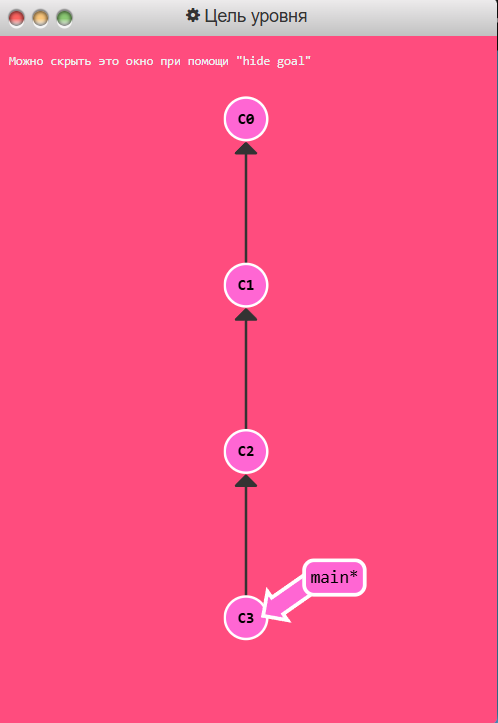
\includegraphics[width=0.4\textwidth]{images/gitbranch1.png}
\caption{Выполнение задания по созданию двух коммитов}
\label{fig:commit_task}
\end{figure}

\section{Урок 2. Ветвление в Git}

Вторая часть обучения на платформе \texttt{Learn Git Branching} была посвящена концепции ветвления.

Ветви (\textit{branches}) в Git являются лёгкими указателями на коммиты. По сути, это просто имена, указывающие на конкретные точки в истории изменений. Благодаря этой простоте ветки создаются и переключаются практически мгновенно, не занимая дополнительных ресурсов.
Такой подход помогает организовать параллельную работу над несколькими задачами без риска затронуть основную рабочую ветку.

\subsection*{Задание}

В рамках упражнения нужно было выполнить две основные команды:
\begin{itemize}
    \item \texttt{git branch} — создать новую ветку с именем \texttt{feature};
    \item \texttt{git checkout} — переключиться на новую ветку.
\end{itemize}

После выполнения команды \texttt{checkout}, указатель \texttt{HEAD} начинает ссылаться на новую ветку, и последующие коммиты будут записываться в её историю.

\subsection*{Результат}

Ниже представлен скриншот, подтверждающий успешное выполнение задания:

\begin{figure}[H]
\centering
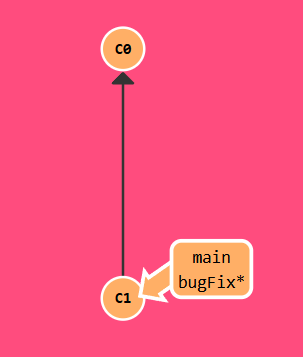
\includegraphics[width=0.4\textwidth]{images/gitbranch2.png}
\caption{Создание и переключение на новую ветку}
\label{fig:gitbranch2}
\end{figure}

\section{Урок 3. Ветки и слияния}

Третье упражнение на платформе \texttt{Learn Git Branching} посвящено механизму объединения изменений, сделанных в разных ветках. В реальных проектах часто бывает, что разработчики работают параллельно: каждый в своей ветке. После завершения работы возникает необходимость объединить эти изменения. В Git это делается с помощью команды \texttt{git merge}.

\texttt{git merge} создаёт новый \textit{сливающий коммит} (merge commit), который объединяет изменения из двух веток. Такой коммит имеет двух родителей — один указывает на текущее состояние основной ветки, а другой — на ветку, с которой происходит слияние. Это позволяет сохранить обе истории изменений и продолжать разработку в объединённой ветке.

\subsection*{Задание}

Для успешного прохождения уровня нужно было выполнить следующие шаги:

\begin{enumerate}
    \item Создать новую ветку с именем \texttt{bugFix}:
    \texttt{git branch bugFix}
    
    \item Переключиться на неё:
    \texttt{git checkout bugFix}
    
    \item Сделать один коммит в ветке \texttt{bugFix}:
    \texttt{git commit}
    
    \item Вернуться в основную ветку:
    \texttt{git checkout main}
    
    \item Сделать ещё один коммит в \texttt{main}:
    \texttt{git commit}
    
    \item Выполнить слияние ветки \texttt{bugFix} в \texttt{main}:
    \texttt{git merge bugFix}
\end{enumerate}

После выполнения этих команд визуализация дерева коммитов изменилась: появился merge-коммит, у которого два родителя. Это означает, что изменения из обеих веток были успешно объединены.

\subsection*{Результат}

На рисунке ниже показан результат успешного слияния ветки \texttt{bugFix} с веткой \texttt{main}:

\begin{figure}[H]
\centering
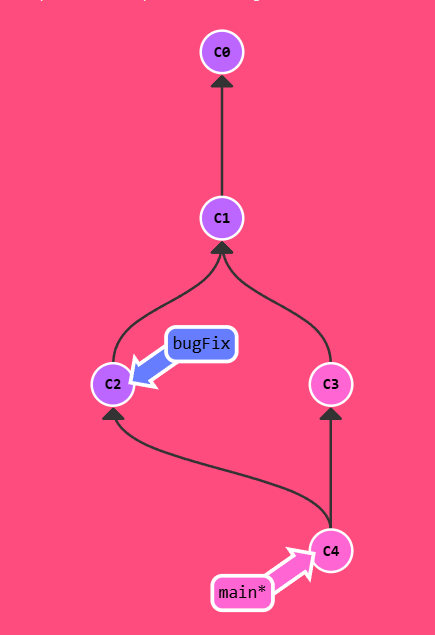
\includegraphics[width=0.4\textwidth]{images/gitbranch3.png}
\caption{Результат слияния ветки \texttt{bugFix} в \texttt{main}}
\label{fig:gitbranch3}
\end{figure}

\section{Урок 4. Git Rebase}

В этом упражнении рассматривался альтернативный способ объединения изменений — \texttt{git rebase}. В отличие от \texttt{merge}, который сохраняет все ветвления и создаёт дополнительный коммит слияния, \texttt{rebase} переписывает историю. Он переносит коммиты одной ветки в конец другой, создавая иллюзию линейной, непрерывной истории разработки.

Главное преимущество \texttt{rebase} — более чистая и читаемая история коммитов. Это особенно полезно при совместной разработке, когда важно понимать, какие изменения в каком порядке были внесены.

\textbf{Важно:} rebase изменяет историю, поэтому его следует применять только к локальным веткам, которые ещё не были опубликованы.

\subsection*{Задание}

Для выполнения задания требовалось сделать следующее:

\begin{enumerate}
    \item Создать ветку \texttt{bugFix}:
    \texttt{git branch bugFix}

    \item Переключиться на ветку \texttt{bugFix}:
    \texttt{git checkout bugFix}
    
    \item Сделать один коммит:
    \texttt{git commit}
    
    \item Перейти на ветку \texttt{main}:
    \texttt{git checkout main}
    
    \item Сделать ещё один коммит в \texttt{main}:
    \texttt{git commit}
    
    \item Снова переключиться на \texttt{bugFix} и выполнить команду:
    \texttt{git rebase main}
\end{enumerate}

В результате коммиты из \texttt{bugFix} были перенесены поверх последних коммитов из ветки \texttt{main}, образовав линейную историю без merge-коммита.

\subsection*{Результат}

На изображении ниже показано дерево после выполнения команды \texttt{rebase}:

\begin{figure}[H]
\centering
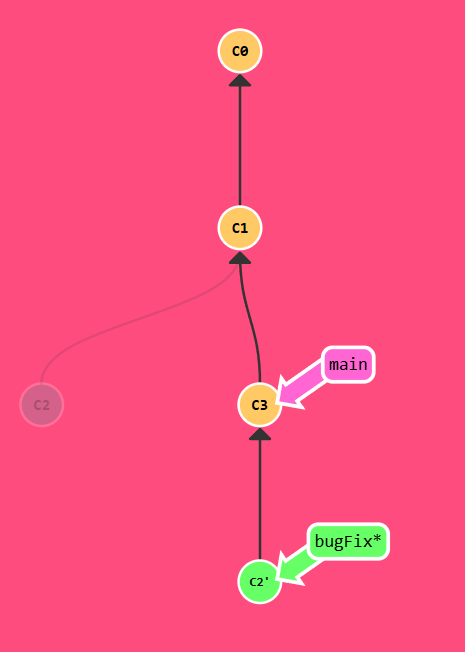
\includegraphics[width=0.4\textwidth]{images/gitbranch4.png}
\caption{Ветка \texttt{bugFix} после rebase на \texttt{main}}
\label{fig:gitbranch4}
\end{figure}

\section{Урок 5. Прогулка по Git и указатель HEAD}

Пятый урок интерактивного курса Learn Git Branching посвящён навигации по дереву коммитов. Понимание структуры коммитов и механизма перемещения по истории изменений — одна из важнейших основ эффективной работы с Git.

\subsection*{Понятие HEAD}

\texttt{HEAD} — это символический указатель на текущий активный коммит. Обычно он указывает на последнюю фиксацию (\textit{commit}) в текущей ветке. При переключении ветки или выполнении команды \texttt{checkout} \texttt{HEAD} изменяется и начинает указывать на другую ветку или конкретный коммит.

Когда \texttt{HEAD} указывает на имя ветки, он «привязан» к этой ветке. При создании коммита вместе с ней обновляется и \texttt{HEAD}. 
Однако Git также позволяет «отцепить» (\textit{detach}) \texttt{HEAD}, напрямую указывая на конкретный коммит по его идентификатору (hash). 
Это полезно, например, для анализа кода или тестирования в прошлых состояниях проекта.

\subsection*{Задание}

Чтобы пройти этот уровень, необходимо:

\begin{enumerate}
    \item Определить идентификатор (hash) последнего коммита в ветке \texttt{bugFix} по визуализации.
    \item Отцепить \texttt{HEAD} от ветки \texttt{bugFix}, указав конкретный коммит напрямую:
    
    \texttt{git checkout c4}
\end{enumerate}

После выполнения команды \texttt{git checkout <hash>} указатель \texttt{HEAD} больше не будет ссылаться на имя ветки — вместо этого он укажет на конкретный коммит. Это называется \textit{detached HEAD} — "отсоединённая голова".

\subsection*{Результат}

На изображении ниже показано, как \texttt{HEAD} был успешно перенаправлен на конкретный коммит по его хешу:

\begin{figure}[H]
\centering
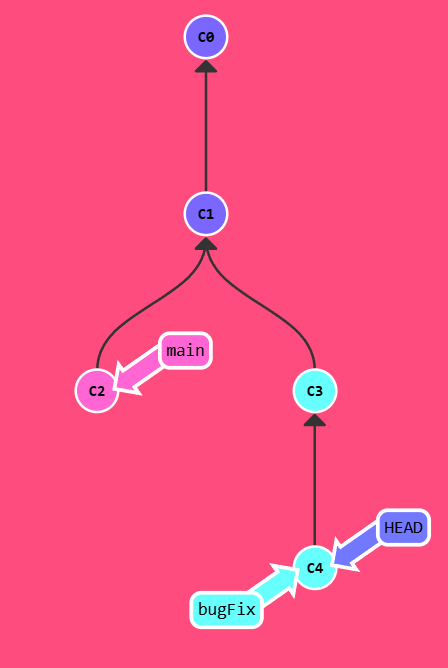
\includegraphics[width=0.4\textwidth]{images/gitbranch5.png}
\caption{HEAD указывает напрямую на коммит по идентификатору}
\label{fig:gitbranch5}
\end{figure}

\section{Урок 6. Относительные ссылки в Git}

В шестом уроке рассматриваются более удобные способы навигации по истории коммитов при помощи относительных ссылок. Работа напрямую с хешами коммитов, особенно длинными, может быть утомительной и неудобной. В реальных проектах идентификаторы коммитов (хеши) могут выглядеть, например, так: \texttt{fed2da64c0efc5293610bdd892f82a58e8cbc5d8}.

К счастью, Git позволяет:

\begin{itemize}
    \item использовать только первые несколько символов хеша — например, \texttt{fed2};
    \item использовать относительные ссылки, которые значительно упрощают навигацию.
\end{itemize}

\subsection*{Относительные ссылки в Git}

Git поддерживает два базовых способа перемещения по истории:

\begin{itemize}
    \item \texttt{\^{}} — переход на первого родителя текущего коммита. Пример: \texttt{HEAD\^{}}
    \item \texttt{\~<n>} — переход на \texttt{n} коммитов назад. Пример: \texttt{HEAD\~2}
\end{itemize}

Также можно использовать относительные ссылки от имени ветки: \texttt{bugFix\^{}}, \texttt{main\~1} и т.д.

\subsection*{Задание}

Для выполнения задания нужно:

\begin{enumerate}
    \item Перейти на первого родителя ветки \texttt{bugFix}, используя относительную ссылку:
    \texttt{git checkout bugFix\^{}}
\end{enumerate}

После выполнения этой команды указатель \texttt{HEAD} будет «отсоединён» и направлен на родительский коммит ветки \texttt{bugFix}.

\subsection*{Результат}

На изображении ниже показано, как \texttt{HEAD} был успешно перемещён на родительский коммит ветки \texttt{bugFix}, с использованием относительной ссылки:

\begin{figure}[H]
\centering
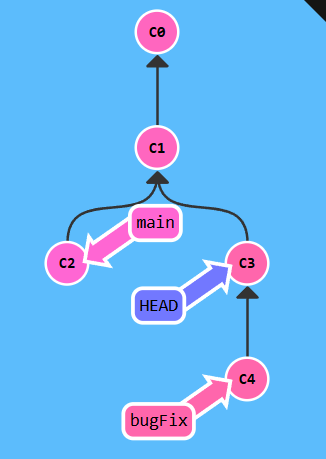
\includegraphics[width=0.4\textwidth]{images/gitbranch6.png}
\caption{Навигация по истории коммитов при помощи относительной ссылки \texttt{bugFix\^{}}}
\label{fig:gitbranch6}
\end{figure}

\section{Урок 7. Оператор \texttt{\~{}} и перемещение ветки (branch forcing)}

В этом уроке рассматривался мощный инструмент для работы с историей коммитов — оператор \texttt{\~{}} (тильда), а также практическое применение относительных ссылок для перемещения веток.

\subsection*{Принудительное перемещение ветки (branch forcing)}

Теперь, когда мы умеем ссылаться на коммиты относительно текущего положения, можно использовать эти знания для изменения положения веток. С помощью команды:

\begin{verbatim}
git branch -f main HEAD~3
\end{verbatim}

можно «перепривязать» ветку \texttt{main} к другому коммиту — в данном случае, к тому, что находится на три коммита позади текущего \texttt{HEAD}. Это называется принудительное перемещение ветки, или \textit{branch forcing}.

Такая операция не создаёт новых коммитов, а просто перемещает указатель ветки.

\subsection*{Ход решения}

В рамках упражнения был выполнен следующий набор команд:

\begin{verbatim}
git branch -f main C6
git checkout HEAD~1
git branch -f bugFix HEAD~1
\end{verbatim}

\begin{itemize}
    \item Сначала ветка \texttt{main} была принудительно перемещена к коммиту \texttt{C6}.
    \item Затем выполнен переход на предыдущий коммит через \texttt{HEAD\~1}.
    \item Ветка \texttt{bugFix} также была перемещена на одну позицию назад от текущего HEAD.
\end{itemize}

\subsection*{Результат}

На рисунке ниже представлен результат выполнения операции перемещения веток с использованием относительных ссылок:

\begin{figure}[H]
\centering
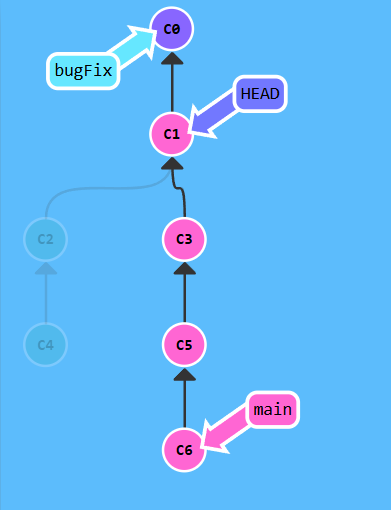
\includegraphics[width=0.4\textwidth]{images/gitbranch7.png}
\caption{Принудительное перемещение веток \texttt{main} и \texttt{bugFix} с помощью относительных ссылок}
\label{fig:gitbranch7}
\end{figure}

\section{Урок 8. Отмена изменений в Git}

Git предоставляет множество способов для отмены изменений, которые уже были зафиксированы в истории репозитория. Эти методы варьируются от работы с отдельными строками до полной отмены коммитов. В этом упражнении фокус был сделан на **высокоуровневых командах** для отмены изменений.

\subsection*{Git reset и Git revert}

Существует два основных способа отката изменений:

\begin{itemize}
    \item \texttt{git reset} — откатывает текущую ветку к предыдущему коммиту, эффективно удаляя последний коммит. 
    Эта операция изменяет историю и применяется в локальных ветках.
    \item \texttt{git revert} — создаёт новый коммит, отменяющий изменения, внесённые предыдущим коммитом. История при этом сохраняется. 
    Применяется, как правило, для отката уже опубликованных изменений.
\end{itemize}

\subsection*{Цель упражнения}

Чтобы пройти этот уровень, необходимо:

\begin{itemize}
    \item Отменить последний коммит на ветке \texttt{local} с помощью \texttt{git reset}:
    \texttt{git reset local}
    \item Отменить последний коммит на ветке \texttt{pushed} с помощью \texttt{git revert}:
    \texttt{git checkout pushed; git revert pushed}
\end{itemize}

\subsection*{Результат}

На рисунке ниже показан результат выполнения команд, иллюстрирующий различие между \texttt{reset} и \texttt{revert}:

\begin{figure}[H]
\centering
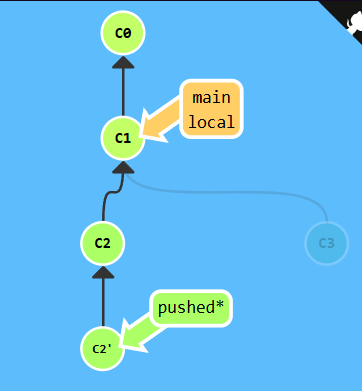
\includegraphics[width=0.4\textwidth]{images/gitbranch8.png}
\caption{Откат изменений: \texttt{reset} удаляет коммит, \texttt{revert} создаёт обратный}
\label{fig:gitbranch8}
\end{figure}

\section{Урок 9. Git Cherry-pick}

В этом уроке изучалась команда \texttt{git cherry-pick}, предназначенная для выборочного применения коммитов из других веток или частей истории 
к текущей позиции HEAD. Это один из самых прямолинейных способов «вытянуть» нужные изменения, не сливая полностью другие ветки.

\subsection*{Что делает git cherry-pick}

Команда:

\begin{verbatim}
git cherry-pick <Commit1> <Commit2> <...>
\end{verbatim}

создаёт новые коммиты на текущей ветке, копируя изменения, содержащиеся в указанных коммитах. Это особенно полезно, когда:

\begin{itemize}
    \item Нужно взять только часть изменений из другой ветки
    \item Не хочется делать слияние всей ветки
    \item Нужно воспроизвести конкретные багфиксы или фичи на другой ветке
\end{itemize}

\subsection*{Цель задания}

Визуализация уровня подсказывала, какие именно коммиты нужно было перенести. Задание состояло в том, чтобы:

\begin{itemize}
    \item Перейти на ветку \texttt{main}
    \item Скопировать изменения из трёх указанных коммитов (\texttt{c3}, \texttt{c4}, \texttt{c7}) в \texttt{main}, используя \texttt{git cherry-pick}
\end{itemize}

\subsection*{Ход решения}

Для прохождения уровня была выполнена следующая команда:

\begin{verbatim}
git cherry-pick c3 c4 c7
\end{verbatim}

\subsection*{Результат}

\begin{figure}[H]
\centering
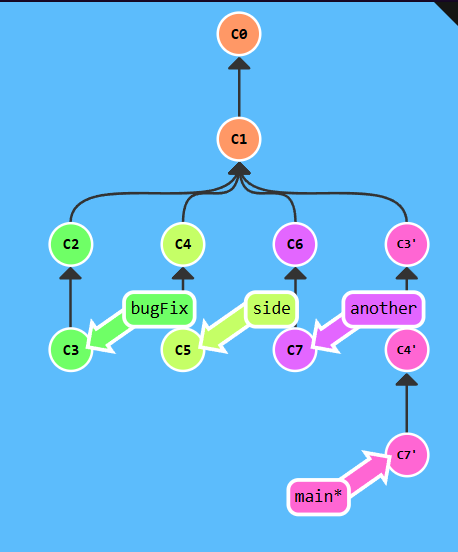
\includegraphics[width=0.4\textwidth]{images/gitbranch9.png}
\caption{Перенос изменений c3, c4 и c7 в main через \texttt{git cherry-pick}}
\label{fig:gitbranch9}
\end{figure}

\section{Урок 10. Git Interactive Rebase}

В этом уроке рассматривался продвинутый инструмент Git — \textbf{интерактивный rebase}, позволяющий гибко управлять порядком, включением или исключением коммитов. Это особенно полезно, когда необходимо:

\begin{itemize}
    \item изменить порядок коммитов;
    \item удалить ненужные коммиты;
    \item объединить несколько коммитов в один (squash);
    \item переписать историю коммитов перед публикацией.
\end{itemize}

\subsection*{Что такое интерактивный rebase}

При запуске команды:

\begin{verbatim}
git rebase -i HEAD~N
\end{verbatim}

Git откроет список из последних \texttt{N} коммитов в редакторе. Пользователь может изменить:

\begin{itemize}
    \item \texttt{pick} на \texttt{drop} — удалить коммит;
    \item порядок строк — переставить коммиты;
    \item объединить коммиты при помощи \texttt{squash} (не использовалось в этом упражнении).
\end{itemize}

\subsection*{Цель упражнения}

Задание заключалось в следующем:

\begin{itemize}
    \item Переставить и отфильтровать коммиты таким образом, чтобы в истории остались только следующие: \texttt{c0, c1, c3, c4, c5}
    \item Удалить из истории коммит \texttt{c2}
    \item Изменить порядок остальных коммитов по примеру
\end{itemize}

\subsection*{Ход выполнения}

В редакторе интерактивного ребейза были выполнены следующие действия:

\begin{figure}[H]
\centering
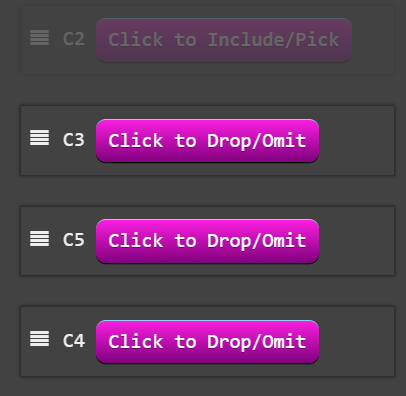
\includegraphics[width=0.4\textwidth]{images/gitbranch10_1.png}
\caption{Комит \texttt{c2} удалён, остальные раствавлены в нужном порядке}
\label{fig:gitbranch10_1}
\end{figure}

\subsection*{Результат}


\begin{figure}[H]
\centering
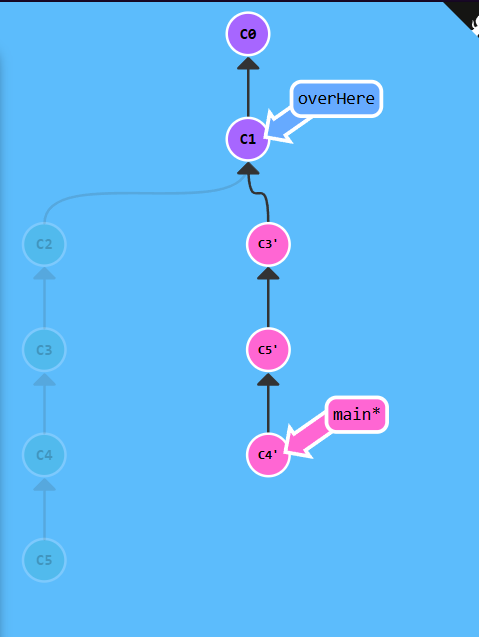
\includegraphics[width=0.4\textwidth]{images/gitbranch10_2.png}
\label{fig:gitbranch10_2}
\end{figure}

\section{Урок 11. Выборочное извлечение нужного коммита}

\subsection*{Ход выполнение}

\begin{itemize}
    \item Использовать \texttt{git rebase -i main}, чтобы из ветки \texttt{bugFix} оставить только коммит \texttt{c4}, содержащий исправление ошибки.
    \item После очистки ветки \texttt{bugFix}, использовать \texttt{git rebase bugFix main}, чтобы аккуратно перенести только нужный коммит в ветку \texttt{main}.
\end{itemize}

\begin{figure}[H]
\centering
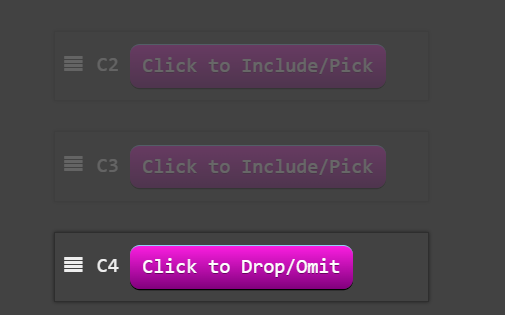
\includegraphics[width=0.4\textwidth]{images/gitbranch11_1.png}
\caption{Фото rebase}
\label{fig:gitbranch11_1}
\end{figure}

\subsection*{Результат}

Ветка \texttt{main} получила только нужный коммит \texttt{c4}, в то время как все отладочные коммиты были отброшены и не попали в основную ветку разработки.

\begin{figure}[H]
\centering
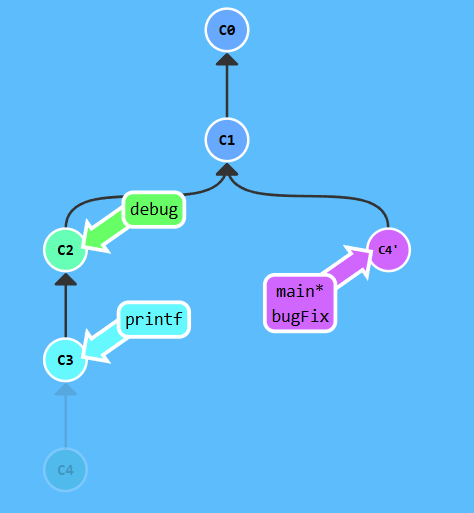
\includegraphics[width=0.4\textwidth]{images/gitbranch11_2.png}
\caption{Выборочное добавление коммита \texttt{c4} в ветку \texttt{main} через rebase}
\label{fig:gitbranch11}
\end{figure}

\section{Урок 12. Жонглируем коммитами}

Этот урок посвящён тонкому управлению историей Git: как изменить содержимое уже созданного (и не самого последнего!) коммита. Это важный приём, когда необходимо внести исправление в старый коммит, не нарушая целостность истории.


В данном уровне нужно отредактировать \texttt{caption}, хотя он находится *под* коммитом \texttt{newImage}. 
Для этого приходится «переиграть» историю.

\begin{figure}[H]
\centering
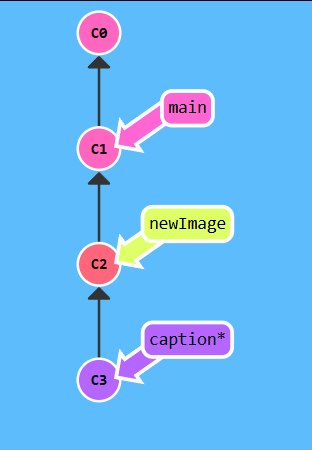
\includegraphics[width=0.4\textwidth]{images/gitbranch12.png}
\caption{исходные данные}
\label{fig:gitbranch12}
\end{figure}

\subsection*{Решение}

\begin{enumerate}
    \item Переставили коммит \texttt{caption} наверх:
    \begin{verbatim}
git rebase -i HEAD~2 # Поменяли местами C3,C2
    \end{verbatim}
    
    \item Отредактировали содержимое коммита с помощью:
    \begin{verbatim}
git commit --amend
    \end{verbatim}
    
    \item Вернули коммиты в исходный порядок:
    \begin{verbatim}
git rebase -i HEAD~2
    \end{verbatim}
    
    \item Переместили ветку \texttt{main} на актуальную часть истории:
    \begin{verbatim}
git rebase caption main
    \end{verbatim}
\end{enumerate}

\subsection*{Результат}

Ветка \texttt{main} теперь включает отредактированный коммит \texttt{caption}, при этом структура истории остаётся линейной и понятной.

\begin{figure}[H]
\centering
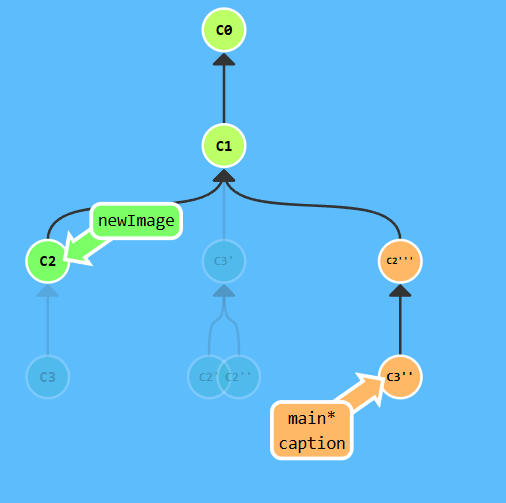
\includegraphics[width=0.4\textwidth]{images/gitbranch12_1.png}
\caption{Редактирование старого коммита с помощью \texttt{rebase} и \texttt{amend}}
\label{fig:gitbranch12}
\end{figure}

\section{Урок 13. Жонглируем коммитами №2 (через \texttt{cherry-pick})}

В этом задании стояла цель достичь того же результата, что и в предыдущем уроке, но без использования интерактивного rebase. 
Вместо этого предлагалось использовать альтернативные команды Git — в частности, \texttt{git cherry-pick} и \texttt{git commit --amend}.

\subsection*{Ход выполнения}

\begin{enumerate}
    \item Перешёл на ветку \texttt{main}:
    \begin{verbatim}
git checkout main
    \end{verbatim}

    \item Взял коммит \texttt{C2} и применил его:
    \begin{verbatim}
git cherry-pick C2
    \end{verbatim}

    \item Внёс исправления в только что применённый коммит с помощью:
    \begin{verbatim}
git commit --amend
    \end{verbatim}

    \item Применил коммит \texttt{C3}, чтобы восстановить порядок:
    \begin{verbatim}
git cherry-pick C3
    \end{verbatim}
\end{enumerate}

\subsection*{Пояснение}

Команда \texttt{git cherry-pick} позволяет избирательно переносить коммиты между ветками или на текущую позицию HEAD. Это удобно, когда необходимо сохранить порядок, но модифицировать определённые шаги.

В отличие от \texttt{rebase -i}, данный подход требует явного управления историей вручную, что может быть даже более прозрачно и гибко в некоторых случаях.

\subsection*{Результат}

Структура дерева коммитов получилась идентичной предыдущему упражнению, с той лишь разницей, что вместо интерактивного ребейза использовалось ручное "жонглирование" с помощью \texttt{cherry-pick} и \texttt{amend}.

\begin{figure}[H]
\centering
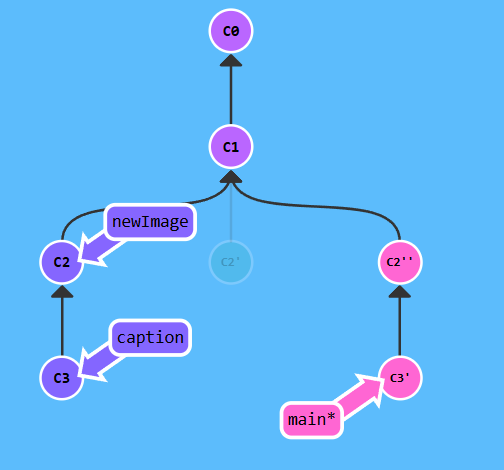
\includegraphics[width=0.4\textwidth]{images/gitbranch13.png}
\caption{Результат жонглирования коммитами через \texttt{git cherry-pick}}
\label{fig:gitbranch13}
\end{figure}

\section{Урок 14. Теги в Git}

До этого момента мы изучали ветки как основной способ ссылаться на определённые коммиты. Однако ветки динамичны: они могут легко передвигаться и изменяться.
Это делает их не лучшим способом «зафиксировать» важные моменты в истории проекта, например, релизы.

\subsection*{Зачем нужны теги?}

Теги (\textit{tags}) в Git — это постоянные метки, указывающие на определённый коммит. 
В отличие от веток, теги не изменяются, их нельзя сдвинуть, и они служат в качестве «якоря» в истории.

Теги особенно полезны для:
\begin{itemize}
    \item обозначения стабильных версий (v1.0, v2.3.1 и т.д.),
    \item возврата к точке релиза или важного изменения,
    \item публикации в открытом доступе.
\end{itemize}

\subsection*{Цель урока}

Создать два тега:
\begin{itemize}
    \item \texttt{v0} указывает на коммит \texttt{C1},
    \item \texttt{v1} указывает на коммит \texttt{C2}.
\end{itemize}

Затем выполнить переход на тег \texttt{v1}, чтобы увидеть состояние проекта на момент этого коммита. Это приведёт к состоянию \textit{detached HEAD}, поскольку нельзя делать коммиты прямо в тег.

\subsection*{Решение}

\begin{verbatim}
git checkout C2
git tag v1 C2
git tag v0 C1
\end{verbatim}

После выполнения этих команд:

\begin{itemize}
    \item Коммит \texttt{C1} помечен тегом \texttt{v0},
    \item Коммит \texttt{C2} — тегом \texttt{v1},
    \item HEAD указывает на \texttt{v1}, но не на какую-либо ветку (detached HEAD).
\end{itemize}

\subsection*{Результат}

\begin{figure}[H]
\centering
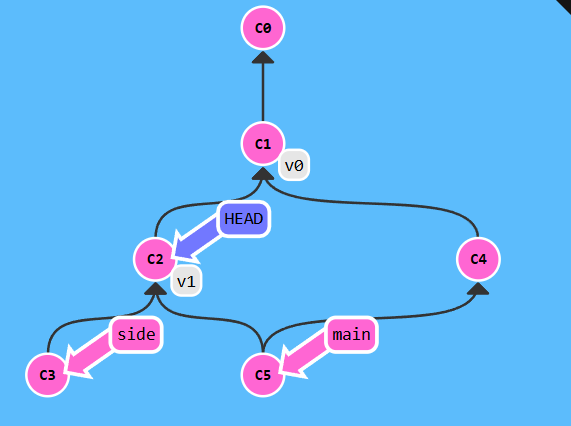
\includegraphics[width=0.4\textwidth]{images/gitbranch14_1.png}
\caption{Создание и переход к тегам в Git}
\label{fig:gitbranch14}
\end{figure}

\section{Урок 15. Команда \texttt{git describe}}

Команда \texttt{git describe} — полезный инструмент Git, который позволяет определить, где именно в истории коммитов вы находитесь по отношению к ближайшему тегу.
Это особенно удобно после работы с такими командами, как \texttt{git bisect}, или при ручной навигации по истории.

\subsection*{Формат вывода}

При вызове команды \texttt{git describe <ref>} Git возвращает строку формата:

\begin{itemize}
    \item \texttt{<tag>} — ближайший тег, найденный в истории коммитов;
    \item \texttt{<numCommits>} — количество коммитов от тега до текущего состояния;
    \item \texttt{<hash>} — сокращённый хеш текущего коммита.
\end{itemize}

Если не указать \texttt{ref}, Git будет использовать текущий \texttt{HEAD}.

\subsection*{Примеры}

В этом упражнении были опробованы следующие команды:

\begin{verbatim}
git describe main
git describe side
git describe bugFix
\end{verbatim}

Каждая команда показала расстояние текущей позиции ветки до ближайшего тега. Это помогает понять, в какой части истории находится ветка, особенно если вы работаете с длинной цепочкой коммитов.

\subsection*{Заключение}

После того как были выполнены команды \texttt{git describe} на нескольких ветках, был сделан дополнительный коммит, чтобы пройти уровень.

\begin{figure}[H]
\centering
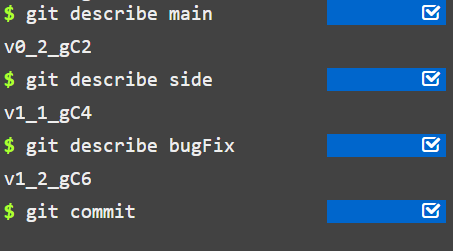
\includegraphics[width=0.4\textwidth]{images/gitbranch15.png}
\caption{Пример использования \texttt{git describe} для определения расстояния до ближайшего тега}
\label{fig:gitbranch15}
\end{figure}

\section{Урок 16. Rebase на нескольких ветках}

В этом упражнении было необходимо выполнить цепочку операций \texttt{rebase} для нескольких веток так, чтобы итоговая история коммитов стала линейной и строго упорядоченной. Это требование особенно важно в больших проектах, где история должна быть чистой, понятной и предсказуемой.

\begin{figure}[H]
\centering
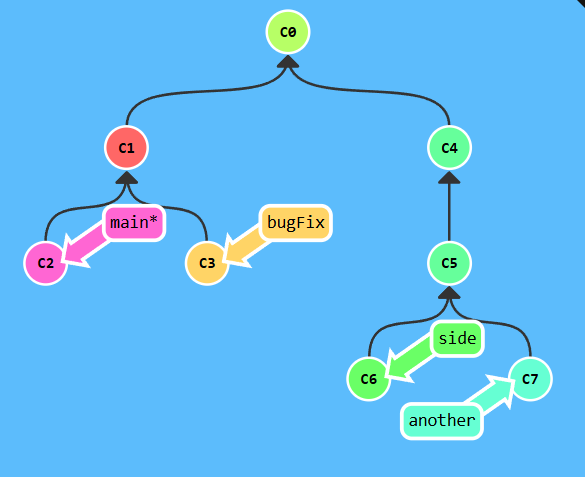
\includegraphics[width=0.4\textwidth]{images/gitbranch16.png}
\caption{исходные данные}
\label{fig:gitbranch16}
\end{figure}

Цель — объединить все изменения из этих веток в ветку \texttt{main}, но не с помощью \texttt{merge}, а строго через \texttt{rebase}, сохранив при этом строгий порядок коммитов: \texttt{C6'}, затем \texttt{C7'}, и так далее.

\subsection*{Решение}

Для достижения цели использовалась последовательность следующих команд:

\begin{verbatim}
git rebase main bugFix
git rebase bugFix side
git rebase side another
git rebase another main
\end{verbatim}

Эти действия:
\begin{enumerate}
    \item Перенесли ветку \texttt{bugFix} поверх \texttt{main},
    \item Затем ветку \texttt{side} поверх \texttt{bugFix},
    \item Затем ветку \texttt{another} поверх \texttt{side},
    \item И, наконец, весь стек веток — обратно в \texttt{main}.
\end{enumerate}

Такой подход гарантирует, что каждый коммит будет находиться строго после предыдущего, сохраняя нужный порядок.

\subsection*{Результат}

На изображении \ref{fig:gitbranch16_1} видно, как история проекта стала линейной благодаря последовательному применению \texttt{rebase} к каждой ветке.

\begin{figure}[H]
\centering
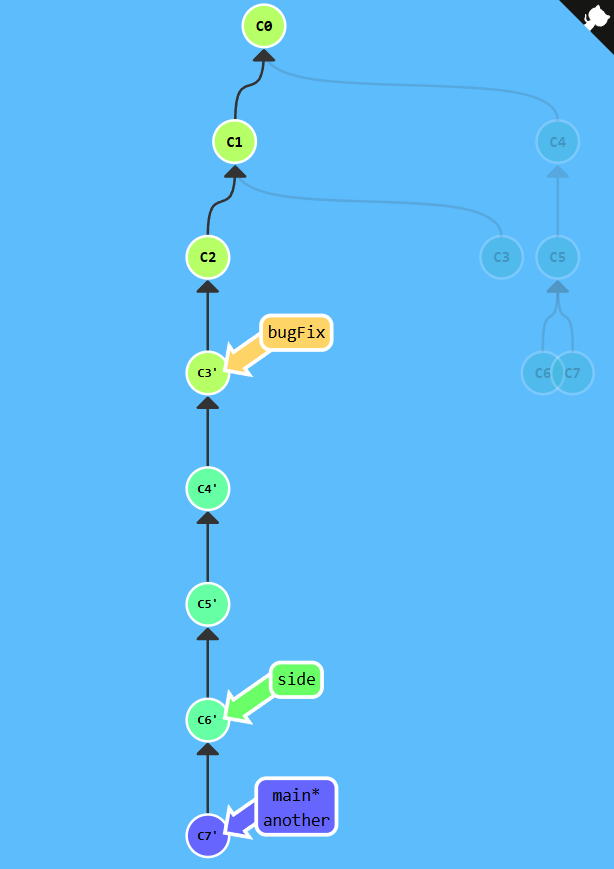
\includegraphics[width=0.4\textwidth]{images/gitbranch16_1.png}
\caption{Последовательный \texttt{rebase} нескольких веток на \texttt{main}}
\label{fig:gitbranch16_1}
\end{figure}

\section{Урок 17. Определение родителей коммита}

Git предоставляет гибкие способы навигации по дереву коммитов. В дополнение к тильде (\texttt{\~{}}), 
которая используется для перемещения назад по цепочке коммитов, также существует оператор каретки (\texttt{\^}),
позволяющий указать конкретного родителя коммита.

\subsection*{Навигация по родителям}

В случае merge-коммитов (слияний), у которых обычно два родителя, Git по умолчанию переходит к первому родителю при использовании \texttt{\^}. Однако, добавляя цифру после каретки, можно выбрать, к какому родителю перейти:

\begin{itemize}
    \item \texttt{HEAD\^} — первый родитель (по умолчанию),
    \item \texttt{HEAD\^2} — второй родитель.
\end{itemize}

Это особенно полезно при анализе истории, откате изменений или создании новых веток от нужного состояния дерева коммитов.

\subsection*{Решение}

В качестве решения использована следующая команда:

\begin{verbatim}
git branch bugWork HEAD~^2~
\end{verbatim}

Она означает следующее:
\begin{enumerate}
    \item \texttt{HEAD\^2{}} — перейти ко второму родителю текущего коммита;
    \item \texttt{\~{}} — перейти на один коммит назад от выбранного родителя;
    \item создать ветку \texttt{bugWork} в этом положении.
\end{enumerate}

\subsection*{Результат}

На рисунке \ref{fig:gitbranch17} показано, где создаётся ветка \texttt{bugWork} после выполнения команды.

\begin{figure}[H]
\centering
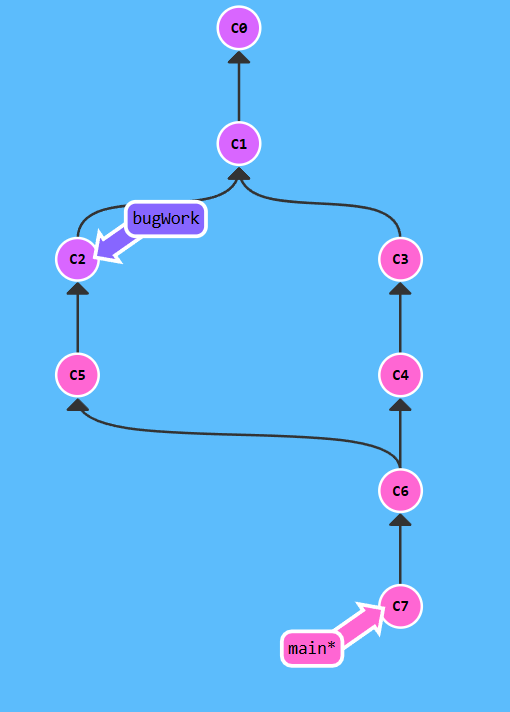
\includegraphics[width=0.4\textwidth]{images/gitbranch17.png}
\caption{Ветка \texttt{bugWork}, созданная с использованием \texttt{\^2{}} и \texttt{\~{}}}
\label{fig:gitbranch17}
\end{figure}

\section{Урок 18. Спутанные ветки}

Этот уровень представляет собой усложнённую задачу по манипуляции ветками в Git. У нас есть три ветки: \texttt{one}, \texttt{two} и \texttt{three}, каждая из которых нуждается в переработке истории коммитов. Вместо простого ребейза здесь применяются инструменты ручного управления — \texttt{cherry-pick} и \texttt{branch -f}.

\subsection*{Описание проблемы}

\begin{itemize}
    \item Ветка \texttt{one} требует изменения порядка коммитов и удаления коммита \texttt{C5}.
    \item Ветка \texttt{two} должна включать все коммиты в новом порядке.
    \item Ветка \texttt{three} должна быть перемещена к одному конкретному коммиту — \texttt{C2}.
\end{itemize}

\begin{figure}[H]
\centering
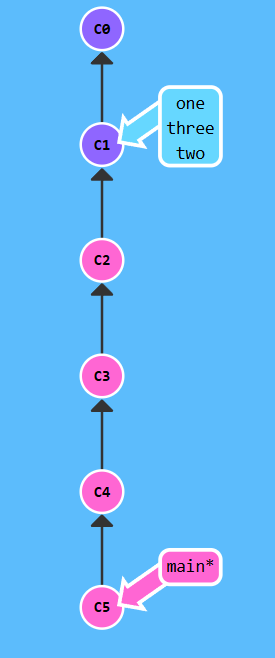
\includegraphics[width=0.4\textwidth]{images/gitbranch18.png}
\caption{Исходные данные}
\label{fig:gitbranch18}
\end{figure}

\subsection*{Решение задачи}

\textbf{Шаг 1.} Изменение ветки \texttt{one}:
\begin{verbatim}
git checkout one
git cherry-pick C4 C3 C2
\end{verbatim}

\textbf{Шаг 2.} Изменение ветки \texttt{two}:
\begin{verbatim}
git checkout two
git cherry-pick C5 C4 C3 C2
\end{verbatim}

\textbf{Шаг 3.} Жёсткое перемещение ветки \texttt{three}:
\begin{verbatim}
git branch -f three C2
\end{verbatim}

\subsection*{Результат}

Ветка \texttt{one} теперь содержит только \texttt{C4, C3, C2}, без \texttt{C5}.  
Ветка \texttt{two} включает \texttt{C5, C4, C3, C2} в указанном порядке.  
Ветка \texttt{three} указывает строго на \texttt{C2}.

\begin{figure}[H]
\centering
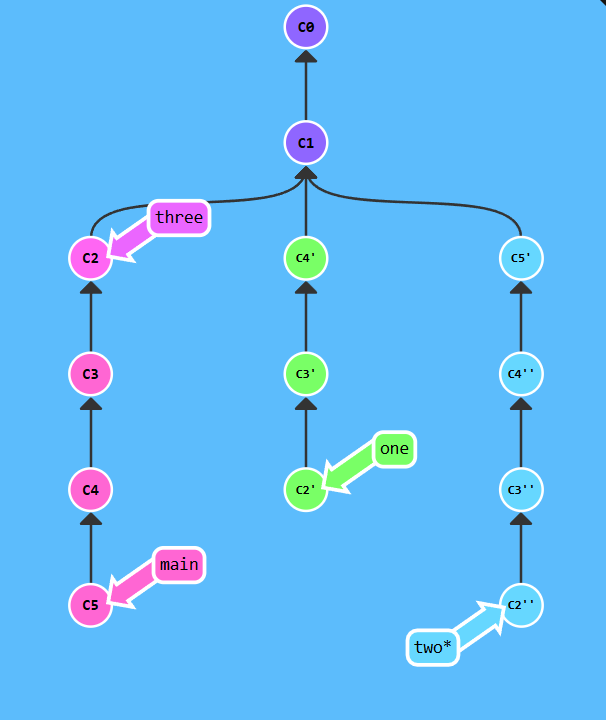
\includegraphics[width=0.4\textwidth]{images/gitbranch18_1.png}
\caption{Обновлённые ветки \texttt{one}, \texttt{two} и \texttt{three} после cherry-pick и переопределения}
\label{fig:gitbranch18_1}
\end{figure}

\section{Урок 19. Удалённые репозитории в Git}

Удалённые репозитории в Git — это копии локальных репозиториев, расположенные на других устройствах или серверах,
чаще всего с возможностью подключения через Интернет. Они необходимы для совместной работы над проектами и резервного хранения данных.

\subsection*{Что такое удалённый репозиторий?}

На практике удалённый репозиторий — это не что иное, как точная копия текущего проекта, доступная по сети. 
Самые популярные примеры: GitHub, GitLab, Bitbucket.

\subsection*{Зачем нужны удалённые репозитории?}

\begin{itemize}
    \item \textbf{Резервное копирование.} Все коммиты и история проекта сохраняются в надёжном удалённом хранилище.
    \item \textbf{Совместная работа.} Разработчики могут вносить изменения независимо и синхронизироваться с помощью pull и push.
    \item \textbf{Интеграция с инструментами.} GitHub, GitLab и другие платформы предоставляют графический интерфейс, CI/CD, issue tracker и многое другое.
\end{itemize}

\subsection*{Команда для создания удалённого репозитория}

В реальных условиях команда \texttt{git clone} используется для создания локальной копии уже существующего удалённого репозитория. Однако в рамках симуляции на сайте \texttt{learngitbranching.js.org}, команда \texttt{git clone} делает наоборот — создаёт удалённый репозиторий из текущего локального, чтобы потренироваться в работе с такими хранилищами.

\subsection*{Команда}

\begin{verbatim}
git clone
\end{verbatim}

\subsection*{Итог}

После выполнения этой команды в симуляторе создаётся зеркальный удалённый репозиторий. 
Это позволит в следующих уроках практиковаться с отправкой (\texttt{push}) и получением (\texttt{pull}) изменений.

\begin{figure}[H]
\centering
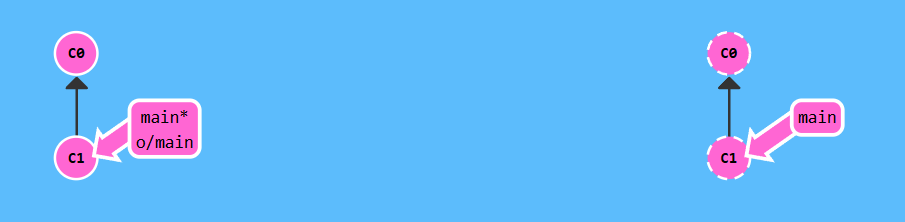
\includegraphics[width=0.0\textwidth]{images/gitbranch19.png}
\caption{Удалённый репозиторий после выполнения команды \texttt{git clone}}
\label{fig:gitbranch19}
\end{figure}

\section{Урок 20. Удалённые ветки в Git}

После знакомства с командой \texttt{git clone} важно понять, что происходит с ветками в локальном репозитории.

\subsection*{Что такое удалённые ветки?}

При выполнении \texttt{git clone} в локальном репозитории появляется новая ветка с именем \texttt{o/main}. 
Такой тип веток называется \textit{удалёнными ветками} и отражает состояние веток на удалённом репозитории.

Удалённые ветки:

\begin{itemize}
    \item Отражают состояние удалённого репозитория на момент последнего обращения к нему.
    \item Позволяют сравнивать локальные изменения с удалёнными.
    \item Не позволяют напрямую работать в них — для внесения изменений необходимо создать локальную ветку.
\end{itemize}

\subsection*{Обозначение удалённых веток}

Имя удалённой ветки всегда состоит из двух частей:

\begin{center}
\texttt{<имя удалённого репозитория>/<имя ветки>}
\end{center}

Например, в ветке \texttt{o/main} \texttt{o} — это имя удалённого репозитория, а \texttt{main} — имя ветки. 
В реальных проектах удалённый репозиторий часто называется \texttt{origin}.

\subsection*{Отделение HEAD при работе с удалёнными ветками}

При переключении на удалённую ветку происходит \textit{detached HEAD} — Git не позволяет делать коммиты прямо в удалённой ветке. 
Для работы нужно создать локальную ветку на основе удалённой.

\subsection*{Задача}

Для выполнения уровня необходимо:

\begin{enumerate}
    \item Сделать один коммит на локальной ветке \texttt{main}.
    \item Переключиться на удалённую ветку \texttt{o/main} (которая будет в состоянии detached HEAD).
    \item Сделать один коммит на ветке \texttt{o/main}.
\end{enumerate}

\begin{figure}[H]
\centering
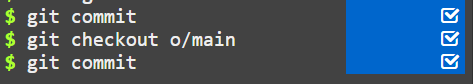
\includegraphics[width=0.4\textwidth]{images/gitbranch20_1.png}
\caption{Команды}
\label{fig:gitbranch20_1}
\end{figure}

Таким образом наглядно видно, как локальные и удалённые ветки взаимодействуют и обновляются.

\begin{figure}[H]
\centering
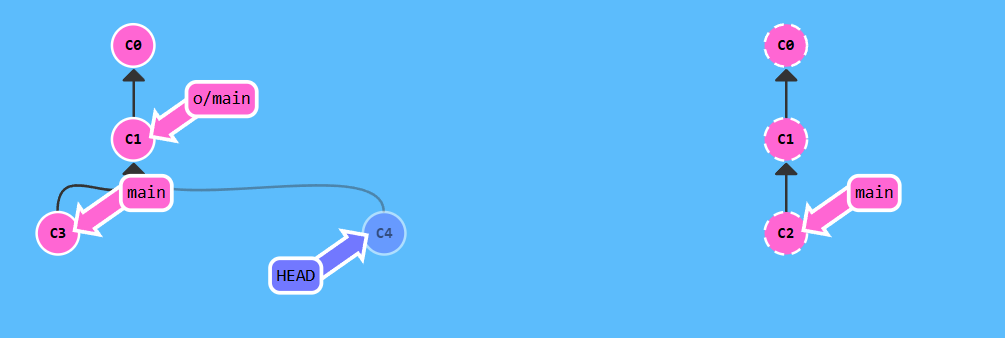
\includegraphics[width=0.7\textwidth]{images/gitbranch20.png}
\caption{Работа с удалёнными ветками \texttt{o/main}}
\label{fig:gitbranch20}
\end{figure}

\section{Урок 21. Git Fetch}

\subsection*{Введение}

Работа с удалёнными репозиториями Git сводится к обмену данными между локальным и удалённым репозиториями. 
Это позволяет делиться изменениями, файлами, идеями и другими важными обновлениями.

В этом уроке мы познакомимся с командой \texttt{git fetch}, которая отвечает за извлечение данных из удалённого репозитория.

\subsection*{Что делает команда \texttt{git fetch}?}

Команда \texttt{git fetch} выполняет две основные задачи:

\begin{itemize}
    \item Связывается с указанным удалённым репозиторием и загружает все новые данные, которых ещё нет в локальном репозитории.
    \item Обновляет ссылки на все ветки из удалённого репозитория (например, \texttt{o/main}), синхронизируя локальное представление удалённых репозиториев с актуальным состоянием.
\end{itemize}

Таким образом, \texttt{git fetch} обновляет локальную копию удалённых веток, но не меняет локальные ветки автоматически — для этого потребуется дополнительная команда, например, \texttt{git merge} или \texttt{git pull}.

\subsection*{Цель урока}

Чтобы успешно пройти уровень, необходимо выполнить команду:

\begin{verbatim}
git fetch
\end{verbatim}

Эта команда скачает все новые коммиты с удалённого репозитория и обновит ссылки на удалённые ветки.

\begin{figure}[H]
\centering
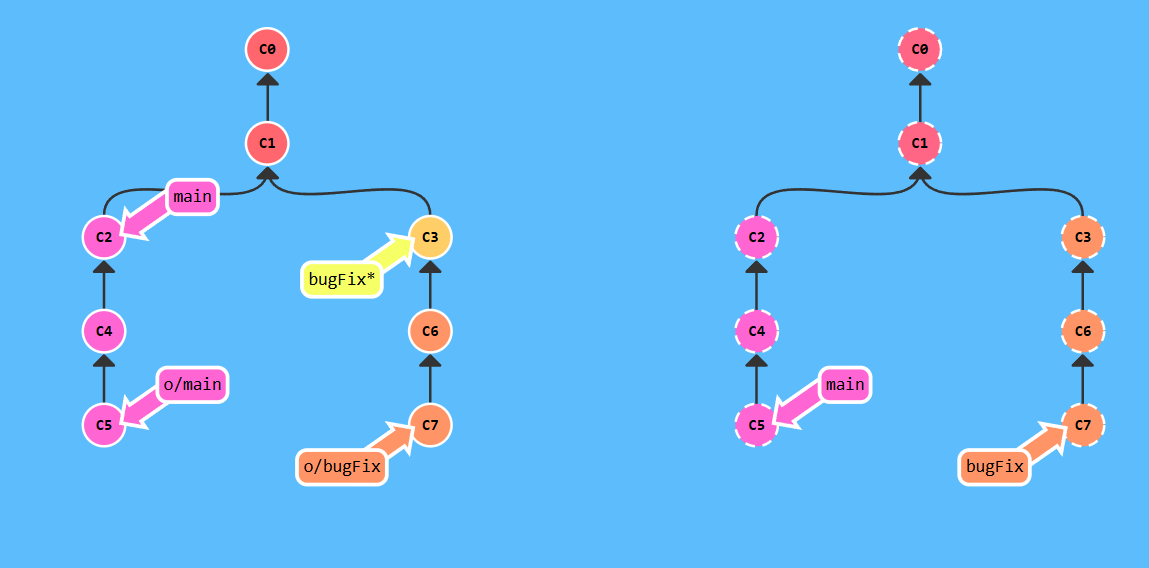
\includegraphics[width=0.7\textwidth]{images/gitbranch21.png}
\caption{Пример обновления удалённых веток после \texttt{git fetch}}
\label{fig:git_fetch}
\end{figure}

\section{Урок 22. Git Pull}

\subsection*{Введение}

После того, как мы научились извлекать данные из удалённого репозитория с помощью команды \texttt{git fetch}, следующий логичный шаг — обновить локальную работу, чтобы отобразить эти изменения.

\subsection*{Объединение изменений}

Получив новые коммиты с удалённого репозитория, можно объединить их с локальной веткой несколькими способами:

\begin{itemize}
  \item \texttt{git cherry-pick o/main} — применить изменения из конкретного коммита;
  \item \texttt{git rebase o/main} — переместить локальные коммиты поверх удалённой ветки;
  \item \texttt{git merge o/main} — объединить удалённую ветку с локальной.
\end{itemize}

Эти операции позволяют интегрировать обновления из удалённого репозитория в вашу текущую работу.

\subsection*{Команда \texttt{git pull}}

Процедура скачивания изменений (\textit{fetch}) и последующего объединения (\textit{merge}) встречается очень часто. 
Для удобства Git объединяет эти действия в одну команду — \texttt{git pull}.

Таким образом, команда \texttt{git pull} выполняет:

\begin{enumerate}
  \item \texttt{git fetch} — скачивает изменения с удалённого репозитория;
  \item \texttt{git merge} — объединяет эти изменения с текущей локальной веткой.
\end{enumerate}

\subsection*{Цель урока}

Для прохождения уровня достаточно выполнить команду:

\begin{verbatim}
git pull
\end{verbatim}

Эта команда обновляет локальную ветку последними изменениями из удалённого репозитория.

\begin{figure}[H]
\centering
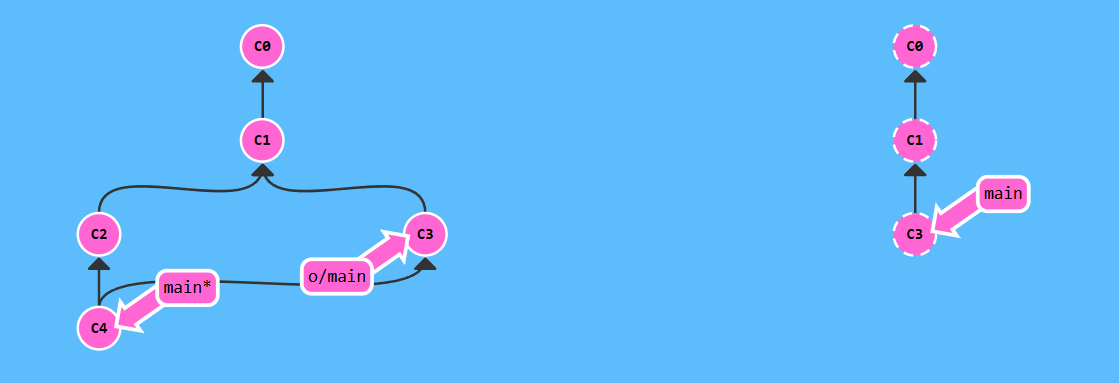
\includegraphics[width=0.7\textwidth]{images/gitbranch22.png}
\caption{Пример работы команды \texttt{git pull}}
\label{fig:git_pull}
\end{figure}

\section{Урок 23. Симуляция совместной работы}

В этом уроке имитируется ситуация, когда удалённый репозиторий изменён другими участниками команды. 
Для отработки навыков синхронизации локальных изменений с удалёнными нам предлагается использовать команду \texttt{git fakeTeamwork}, которая создаёт такие изменения.
Для выполнения задания необходимо:

\begin{enumerate}
    \item Клонировать репозиторий командой \texttt{git clone}.
    \item Смоделировать изменения коллег с помощью \texttt{git fakeTeamwork main 2}.
    \item Сделать локальный коммит.
    \item Выполнить \texttt{git pull} для слияния удалённых изменений с локальными.
\end{enumerate}

Таким образом, этот урок помогает понять, как работать с обновлениями, сделанными другими в удалённом репозитории, и синхронизировать локальную работу.

\begin{figure}[H]
\centering
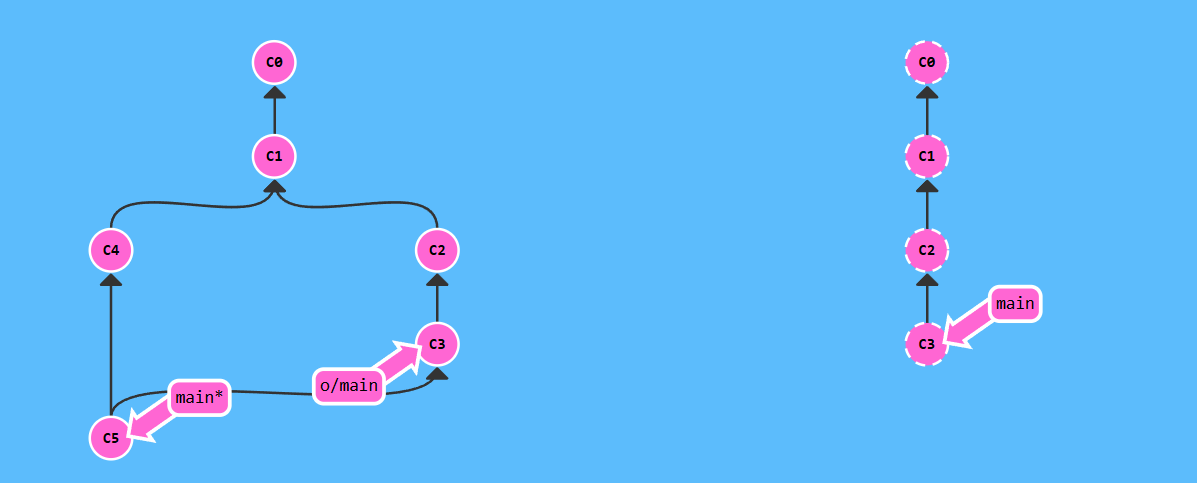
\includegraphics[width=0.7\textwidth]{images/gitbranch23.png}
\caption{Пример симуляции командной работы}
\label{fig:git_pull}
\end{figure}

\section{Урок 24. Git Push}

После того как мы скачали изменения из удалённого репозитория и объединили их с локальными, 
следующим шагом является публикация своих изменений обратно в удалённый репозиторий. Для этого используется команда \texttt{git push}.
Команда \texttt{git push} загружает локальные коммиты в удалённый репозиторий, 
делая их доступными для других участников проекта. Это обратная операция по отношению к \texttt{git pull}.
В ходе урока необходимо было сделать два локальных коммита и выполнить \texttt{git push}, чтобы опубликовать изменения в удалённом репозитории.
Важно учитывать, что поведение \texttt{git push} без аргументов зависит от настройки \texttt{push.default}, 
которая обычно устанавливается в значение \texttt{upstream}.
Таким образом, \texttt{git push} позволяет делиться своей работой и поддерживать проект в актуальном состоянии для всей команды.

\begin{figure}[H]
\centering
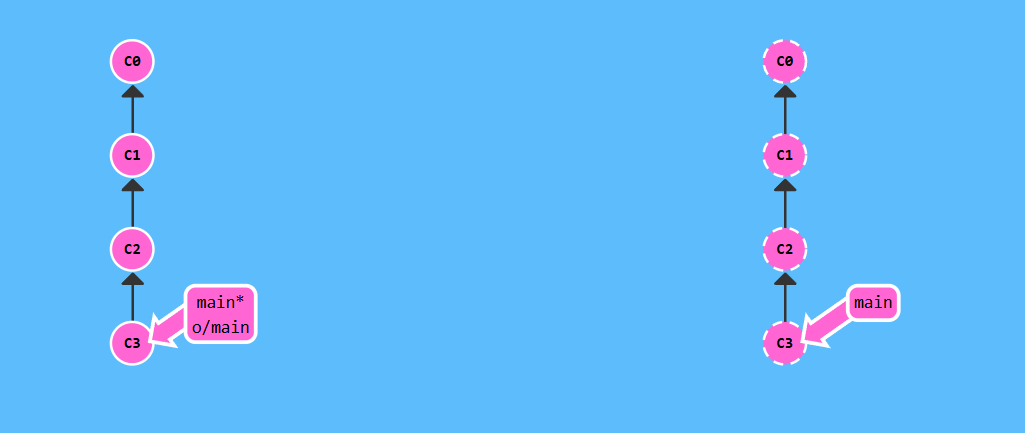
\includegraphics[width=0.7\textwidth]{images/gitbranch24.png}
\caption{Пример Git Push}
\label{fig:git_push}
\end{figure}

\section{Урок 25. Когда наработки расходятся}

В данном уроке мы рассмотрели ситуацию, когда локальные и удалённые наработки расходятся, 
то есть история коммитов в репозиториях не совпадает. Это частая проблема при совместной работе, когда несколько разработчиков вносят изменения параллельно.
Чтобы избежать конфликтов при объединении таких изменений, в уроке была использована команда \texttt{git pull --rebase}, 
которая позволяет "переписать" локальные коммиты поверх обновлённой истории удалённого репозитория. Это помогает сохранить более чистую и линейную историю изменений.

Последовательность действий была следующей:
\begin{itemize}
  \item клонирование репозитория (\texttt{git clone})
  \item имитация изменений в удалённом репозитории (\texttt{git fakeTeamwork})
  \item локальный коммит
  \item обновление локального репозитория с применением ребейза (\texttt{git pull --rebase})
  \item публикация изменений в удалённый репозиторий (\texttt{git push})
\end{itemize}

Таким образом, использование \texttt{git pull --rebase} помогает правильно интегрировать локальные изменения с удалёнными, минимизируя возможные конфликты.

\begin{figure}[H]
\centering
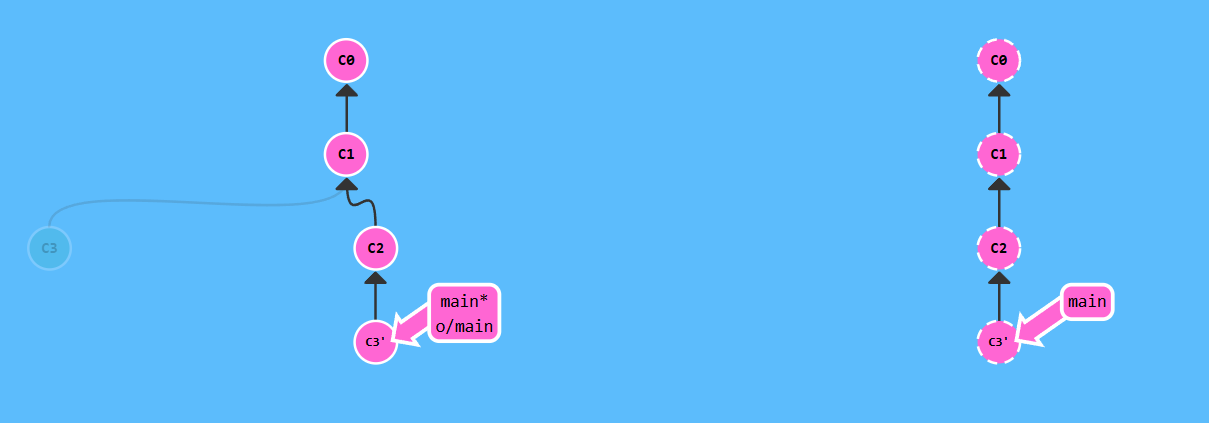
\includegraphics[width=0.7\textwidth]{images/gitbranch25.png}
\caption{}
\label{fig:git_pull_rebase}
\end{figure}

\section{Урок: Remote Rejected!}

В этом уроке рассматривается ситуация, когда при попытке загрузить (push) изменения в ветку \texttt{main} удалённого репозитория возникает ошибка отклонения. Это происходит потому, что в удалённом репозитории для ветки \texttt{main} настроена политика, требующая использовать Pull Request для внесения изменений.

Причины отклонения:
\begin{itemize}
  \item Ветка \texttt{main} заблокирована для прямых изменений.
  \item Все изменения должны вноситься через отдельные ветки и Pull Request.
\end{itemize}

Решение задачи:
\begin{enumerate}
  \item Сбросить локальную ветку \texttt{main} к состоянию удалённой ветки, чтобы синхронизироваться:
  \begin{verbatim}
  git reset --hard o/main
  \end{verbatim}
  \item Создать новую ветку \texttt{feature} на основе коммита \texttt{C2}:
  \begin{verbatim}
  git checkout -b feature C2
  \end{verbatim}
  \item Отправить ветку \texttt{feature} на удалённый репозиторий:
  \begin{verbatim}
  git push origin feature
  \end{verbatim}
\end{enumerate}

Таким образом, мы соблюдаем политику работы с веткой \texttt{main}, используя отдельную ветку для разработки и Pull Request для объединения изменений.

\begin{figure}[H]
\centering
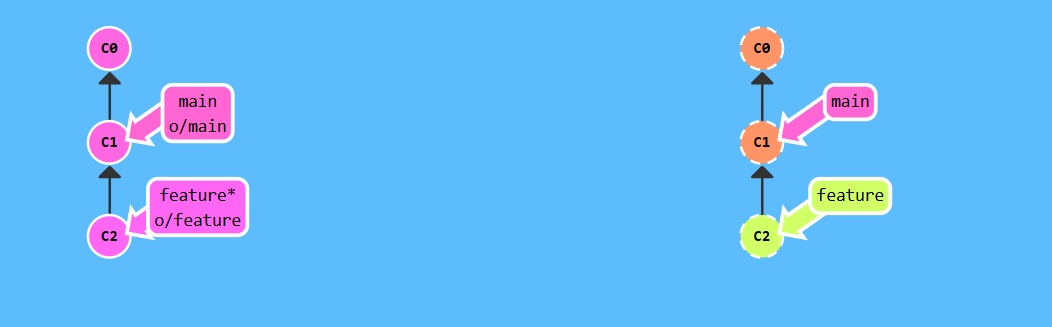
\includegraphics[width=0.7\textwidth]{images/gitbranch26.png}
\caption{Remote Rejected}
\label{fig:gitbranch26}
\end{figure}

\chapterConclusionSection{git_branching_chapter_title}

В ходе выполнения заданий я подробно изучил основные команды и принципы работы с системой контроля версий Git.
Особое внимание я уделил работе с ветками, их созданию, слиянию и перемещению, а также освоил методы управления историей коммитов через rebase 
и cherry-pick. Мне удалось понять, как правильно организовать совместную работу в команде, включая работу с удалёнными репозиториями как скачивать
обновления (fetch, pull), так и отправлять свои изменения (push).
Особенно полезным оказался опыт работы с конфликтами и ситуациями, когда локальные и удалённые версии расходятся.
Я узнал, как правильно восстанавливать состояние веток, создавать новые ветки для разработки новых функций и соблюдать правила работы с защищёнными ветками, используя pull request вместо прямого пуша.
Выполнение практических заданий на сайте learngitbranching.js.org помогло закрепить теоретические знания и увидеть визуальное представление всех операций, 
что значительно упростило понимание. В целом, эта работа позволила мне уверенно ориентироваться в Git, что является важным навыком для эффективной командной разработки и поддержки проектов.

\chapter{Практическое погружение в Git: Git Immersion}\label{gitimmersion_chapter_title}

\section{Lab 1: Настройка Git и Ruby}

\textbf{Цель:} настроить Git и Ruby для начала работы.

Перед началом работы с Git необходимо указать имя и email пользователя, а также настроить поведение с переносами строк. Также потребуется интерпретатор Ruby для последующих лабораторных.

\subsection*{Настройка имени и электронной почты}

Команды, необходимые для глобальной настройки имени и почты:

\begin{minted}{bash}
git config --global user.name "k1tetsssu"
git config --global user.email "sereja.maev05@gmail.com"
\end{minted}

Эти данные будут отображаться в каждом сделанном вами коммите.

\subsection*{Настройка переноса строк}

Для корректной работы с переносами строк:

\textbf{Для пользователей Windows:}

\begin{minted}{bash}
git config --global core.autocrlf true
git config --global core.safecrlf true
\end{minted}

Эти параметры обеспечивают правильное преобразование переносов строк при сохранении файлов, избегая лишних изменений при коммитах.

\subsection*{Установка Ruby}

Для выполнения некоторых лабораторных заданий необходим установленный интерпретатор Ruby.
\textbf{Проверка установки Ruby:}

\begin{minted}{bash}
ruby --version
\end{minted}

Если Ruby установлен корректно, вы увидите версию установленного интерпретатора.

\section*{Вывод}

В данной практической работе я изучил и применил на практике два важных инструмента для работы с документами и кодом --- \LaTeX{} и Git. 
В первой части я освоил основы работы с \LaTeX{}: познакомился с его синтаксисом,
установил необходимое программное обеспечение в среде WSL на Windows и научился создавать хорошо структурированные и
профессионально оформленные документы. Это позволило понять, насколько \LaTeX{} удобен для создания научных и технических текстов с правильным форматированием.
Во второй части я прошёл обучающие уроки по работе с Git, что дало мне понимание,
как эффективно использовать систему контроля версий. Я научился создавать коммиты, работать с ветками, выполнять слияния и ребейзы, 
а также управлять удалёнными репозиториями и совместной работой над проектами. Практические задания помогли закрепить знания и подготовили меня к реальной работе с Git в командной среде.
В целом, данная работа значительно расширила мои навыки в области подготовки документов и контроля версий, что важно для успешной работы над проектами в профессиональной среде.

\end{document}